Im Folgenden werden die notwendigen theoretischen Grundlagen für den Versuch erklärt. Dabei wird zunächst auf die physikalischen Prozesse und anschließend auf die elektronische Umsetzung der Messung eingegangen. 
\subsection{Wechselwirkung ionisierender Strahlung mit Materie}
Die Emission von $\gamma$-Strahlung wird über die Wechselwirkung dieser mit dem jeweiligen Detektormaterial nachgewiesen. Das Grundprinzip ist dabei, dass die Energie des Photons zunächst auf Elektronen übertragen wird und diese dann die Energie an das Detektormaterial abgeben. Im Folgenden werden drei mögliche Wechselwirkungen skizziert.
\subsubsection*{Compton-Effekt} 
Beim Compton-Effekt streut ein Photon an einem Teilchen (siehe Abbildung \ref{fig:compton}). Dabei wird ein gewisser Impuls vom Photon auf das Teilchen übertragen. Abhängig von Ablenkwinkel $\phi$ des gestreuten Photons lässt sich aus der (Vierer-)Impulserhaltung die Wellenlänge des gestreuten Photons zu
\begin{align}
  \lambda-\lambda_0=\frac{h}{mc}(1-\cos \phi)
  \label{eq:compton}
\end{align} 
berechnen. $h$ und $c$ sind dabei das Plancksche Wirkungsquantum und die Lichtgeschwindigkeit. $m$ ist die Masse des Teilchens. Der Ausdruck für die Wellenlängenverschiebung gilt in dem Bezugssystem, in dem das Teilchen zunächst ruht. Nach \cite{wirkungsquerschnitt} ist der Wirkungsquerschnitt direkt proportional zu der Protonenzahl $Z$ der Atome des Materials. Weiter ist der Wirkungsquerschnitt für ein einzelnes Elektron in \cite{wirkungsquerschnitt} beschrieben durch 
\begin{align}
  \diff{\sigma}{\Omega} \propto \left( \frac{\lambda_0}{\lambda} \right)^2 \left( \frac{\lambda_0}{\lambda}+ \frac{\lambda}{\lambda_0}-\sin^2 \phi\right),
\label{eq:compton_cs}
\end{align} 
er wird also maximal für Vorwärts- und Rückwärtsstreuung.
\begin{figure}[h]
  \centering
  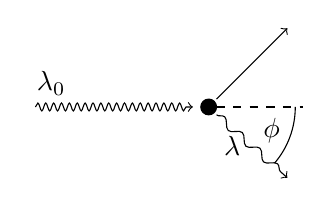
\begin{tikzpicture}[photon1/.style={decorate,decoration={snake, segment length=1mm, amplitude=0.5mm, post length=0.5mm}},photon2/.style={decorate,decoration={snake, segment length=3mm, amplitude=0.5mm, post length=0.5mm}}]
    \draw [->,photon1] (0,2)--(2,2);
    \draw [fill=black] (2.2,2) circle (0.1);
    \draw [->] (2.3,2.1)--(3.2,3);
    \draw [->,photon2] (2.3,1.9)--(3.2,1.1);
    \draw [dashed] (2.3,2)--(3.4,2);
    \draw (0.2,2.3) node {$\lambda_0$}; 
    \draw (2.5,1.5) node {$\lambda$};
    \draw (3.3,2) arc (0:-40.5:1.1);
    \draw (3,1.7) node {$\phi$};
  \end{tikzpicture}
  \caption{Compton-Effekt}
  \label{fig:compton}
\end{figure}

\subsubsection*{Photoeffekt}
Beim Photoeffekt wird die Energie eines einfallenden Photons von einem Hüllenelektron eines Atoms absorbiert. Dadurch wird das Elektron ionisiert. Die kinetische Energie des Elektrons entspricht dann der ursprünglichen Energie des Photons abzüglich der Bindungsenergie des Elektrons. Der Wirkungsquerschnitt bei der Energie $E$ des einfallenden Photons und der Protonenzahl $Z$ des Atoms ist nach \cite{wirkungsquerschnitt} gegeben durch
\begin{align*}
  \sigma \propto \begin{cases}
    Z^4/E^3, & \text{bei niedriger Energie}\\
    Z^5/E, & \text{bei hoher Energie}.
  \end{cases}
\end{align*}
Durch den starken Anstieg des Wirkungsquerschnitts mit der Protonenzahl kann durch die Verwendung von Elementen mit hoher Ordnungszahl eine Dominanz des Photoeffektes bei der Detektion forciert werden.

\subsubsection*{Paarbildung}
Bei der Paarbildung erzeugt ein energiereiches Photon ein Elektron-Positron-Paar. Die überschüssige Energie geht dabei in die kinetische Energie der erzeugten Teilchen. Ein Photon alleine kann noch nicht die Paarbildung auslösen. Es ist die Anwesenheit eines Atomkerns, eines Elektrons oder eines weiteren energiereichen Photons notwendig. Das Photon muss für die Paarbildung mindestens eine Energie haben, die der doppelten Ruheenergie des Elektrons entspricht (Energieerhaltung). Nach \cite{wirkungsquerschnitt} ist der Wirkungsquerschnitt bei kleiner Photonenenergie proportional zu $\ln E$ und bei großer Energie konstant. Bei der Paarproduktion im Feld eines Atomkerns mit Protonenzahl $Z$ ist er außerdem proportional zu $Z^2$, im Feld eines Hüllenelektrons proportional zu $Z$.

\subsection{Szintillationszähler}
Ein Szintillator weist ionisierende Teilchen nach. Die Teilchen regen die Atome im Szintillationsmaterial an. Nach einer mittleren Anregungsdauer fällt das Atom zurück in den Grundzustand und emittiert dabei ein Photon der entsprechenden Wellenlänge. Dieses Photon kann nun auch wieder weitere Atome anregen und es kommt zu einer Art Random-Walk. Um diesen zu unterbrechen, wird das Szintillationsmaterial schwach mit wellenlängenverschiebenden Molekülen dotiert. Trifft ein Photon auf ein solches, wird das Licht zu langwelligerem Licht umgewandelt. Dieses kann nicht vom Szintillator absorbiert werden und somit über einen Lichtleiter zu einer Photodiode gelangen. Diese erzeugt eine messbare elektrische Spannung. Der Prozess ist in Abbildung \ref{fig:szintillator} schematisch skizziert.
\begin{figure}[h]
  \centering
  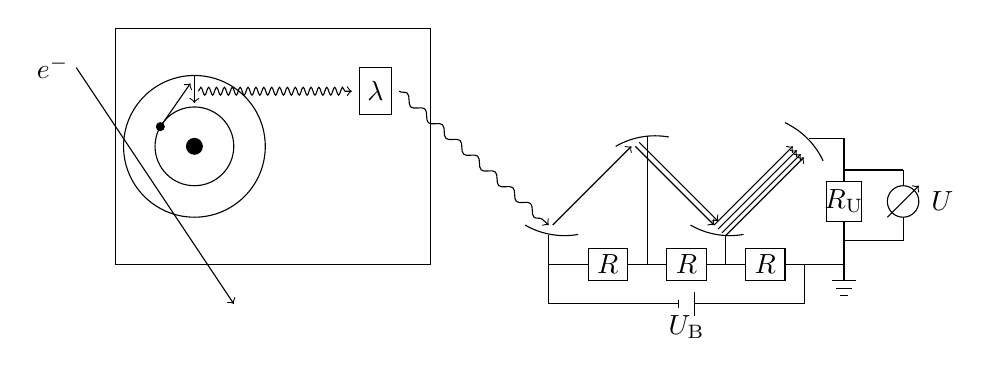
\begin{tikzpicture}[photon1/.style={decorate,decoration={snake, segment length=1mm, amplitude=0.5mm, post length=0.5mm}},photon2/.style={decorate,decoration={snake, segment length=3mm, amplitude=0.5mm, post length=0.5mm}}]
    \draw (0,0) rectangle (4,3);
    \draw [->] (-0.5,2.5)--(1.5,-0.5);
    \draw (-0.8,2.5) node {$e^-$};
    \draw (1,1.5) circle (0.9);
    \draw (1,1.5) circle (0.5);
    \draw [fill=black] (1,1.5) circle (0.1);
    \draw [fill=black] (1-0.5*1.732/2,1.5+1/4) circle (0.05);
    \draw [->] (1-0.5*1.732/2,1.5+1/4)--(0.95,2.3);
    \draw [->] (1,2.4) -- (1,2.05);
    \draw [->,photon1] (1.05,2.2) -- (3,2.2);
    \draw (3.1,1.9) rectangle (3.5,2.5);
    \draw (3.3,2.2) node {$\lambda$};
    \draw [->,photon2] (3.6,2.2)-- (5.5,0.5);
    \draw (5.2,0.5) arc (-120:-80:1);
    \draw [->] (5.55,0.5) -- (6.55,1.5);
    \draw (6.35,1.5) arc (120:80:1);
    \draw [->] (6.6,1.5) -- (7.6,0.5);
    \draw [->] (6.65,1.55) -- (7.65,0.55);
    \draw (7.3,0.5) arc (-120:-80:1);
    \draw [->] (7.65,0.45) -- (8.65,1.45);
    \draw [->] (7.6,0.5) -- (8.6,1.5);
    \draw [->] (7.7,0.4) -- (8.7,1.4);
    \draw [->] (7.74,0.36) -- (8.74,1.36);
    \draw (8.5,1.8) arc (65:25:1);
    \draw (9,0)--(8.5,0);
    \draw (8.75,0)--(8.75,-0.5)--(7.35,-0.5);
    \draw (7.15,-0.5)--(5.5,-0.5)--(5.5,0);
    \draw (8.5,0.2) rectangle (8,-0.2);
    \draw (8.25,0) node {$R$};
    \draw (8,0) -- (7.5,0);
    \draw (7.5,0.2) rectangle (7,-0.2);
    \draw (7.25,0) node {$R$};
    \draw (7,0) -- (6.5,0);
    \draw (7.75,0)--(7.75,0.375);
    \draw (6.75,0)--(6.75,1.635);
    \draw (6.5,0.2) rectangle (6,-0.2);
    \draw (6.25,0) node {$R$};
    \draw (6,0)--(5.5,0)--(5.5,0.375);
    \draw (7.35,-0.65)--(7.35,-0.35);
    \draw (7.15,-0.55)--(7.15,-0.45);
    \draw (7.25,-0.8) node {$U_\mathrm{B}$};
    \draw (9,0)--(9.25,0)--(9.25,0.55);
    \draw (9.03,0.55) rectangle (9.47,1.05);
    \draw (9.25,0.8) node {$R_\mathrm{U}$};
    \draw (9.25,1.05)--(9.25,1.6)--(8.8,1.6);
    \draw (9.25,0)--(9.25,-0.2);
    \draw (9.1,-0.2)--(9.4,-0.2);
    \draw (9.15,-0.3)--(9.35,-0.3);
    \draw (9.2,-0.4)--(9.3,-0.4);
    \draw (9.25,0.3)--(10,0.3);
    \draw (9.25,1.2)--(10,1.2);
    \draw (10,0.8) circle (0.2);
    \draw (10,0.3)--(10,0.6);
    \draw (10,1.2)--(10,1);
    \draw [->] (9.8,0.6)--(10.2,1);
    \draw (10.5,0.8) node {$U$};
  \end{tikzpicture}
  \caption{Beispiel für Signalerzeugung im Szintillator durch Elektron}
  \label{fig:szintillator}
\end{figure}

\subsection{Halbleiterdetektor}
Ein Halbleiterdetektor basiert auf einer in Sperrrichtung betriebenen Halbleiterdiode. Durch die Schaltung in Sperrrichtung entsteht an dem Halbleiterübergang eine ladungsträgerarme Zone, die so genannte Sperrschicht. Die Ausdehnung dieser Sperrschicht hängt von der angelegten Spannung ab. Trifft nun ionisierende Strahlung auf die Sperrschicht werden die Elektronen aus der Bindung gelöst und es entstehen Elektron-Loch-Paare. Durch das elektrische Feld in der Sperrschicht werden Elektronen und Löcher zu jeweils entgegengesetzten Polen gezogen. Somit entsteht kurzzeitig ein Strom welcher über einem Wiederstand als Spannungspuls gemessen werden kann. Der Prozess ist schematisch in Abbildung \ref{fig:halbleiterdetektor} skizziert.

\begin{figure}[h]
  \centering
  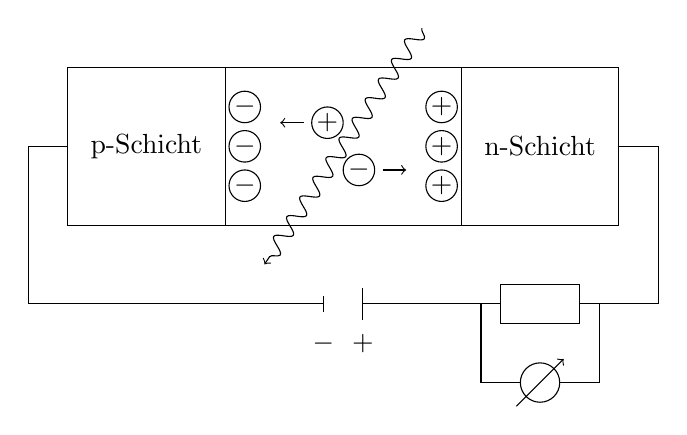
\begin{tikzpicture}[photon/.style={decorate,decoration={snake, segment length=3mm, amplitude=1mm, post length=0.5mm}}]
    \draw (-1,5) rectangle (6,7);
    \draw (1,5)--(1,7);
    \draw (4,5)--(4,7);
    \draw (0,6) node {p-Schicht};
    \draw (5,6) node {n-Schicht};
    \draw (1.25,6.5) circle (0.2);
    \draw (1.25,6.5) node {$-$};
    \draw (1.25,6) circle (0.2);
    \draw (1.25,6) node {$-$};
    \draw (1.25,5.5) circle (0.2);
    \draw (1.25,5.5) node {$-$};
    \draw (3.75,6.5) circle (0.2);
    \draw (3.75,6.5) node {$+$};
    \draw (3.75,6) circle (0.2);
    \draw (3.75,6) node {$+$};
    \draw (3.75,5.5) circle (0.2);
    \draw (3.75,5.5) node {$+$};
    \draw [->,photon] (3.5,7.5)--(1.5,4.5);
    \draw (2.7,5.7) circle (0.2);
    \draw (2.7,5.7) node {$-$};
    \draw [->] (3,5.7)--(3.3,5.7);
    \draw (2.3,6.3) circle (0.2);
    \draw (2.3,6.3) node {$+$};
    \draw [->] (2,6.3)--(1.7,6.3);
    \draw (-1,6)--(-1.5,6)--(-1.5,4)--(2.25,4);
    \draw (6,6)--(6.5,6)--(6.5,4)--(5.5,4);
    \draw (5.5,4.25) rectangle (4.5,3.75);
    \draw (4.5,4)--(2.75,4);
    \draw (2.25,3.9)--(2.25,4.1);
    \draw (2.75,3.8)--(2.75,4.2);
    \draw (2.25,3.5) node {$-$};
    \draw (2.75,3.5) node {$+$};
    \draw (5.75,4)--(5.75,3)--(5.25,3);
    \draw (4.25,4)--(4.25,3)--(4.75,3);
    \draw (5,3) circle (0.25);
    \draw [->] (4.7,2.7)--(5.3,3.3);
  \end{tikzpicture}
  \caption{Strompulserzeugung in Halbleiterdetektor}
  \label{fig:halbleiterdetektor}
\end{figure}

Die Zahl der erzeugten Elektron-Loch-Paare ist proportional zu der abgegebenen Energie des Photons. In diesem Versuch wird ein Halbleiterdetektor aus Germanium verwendet. Germanium ist durch die hohe Ordnungszahl von 32 besonders geeignet, da der Wirkungsquerschnitt für den Photoeffekt so deutlich größer ist als bei Elementen geringerer Ordnungszahlen. Aufgrund der geringen Anregungsenergie (etwa \SI{0.67}{\electronvolt} bei \SI{302}{\kelvin} \cite{bandgap}) muss der Germaniumdetektor allerdings gekühlt werden, da sonst das Signal durch thermische Effekte dominiert werden würde.

\subsection{Signalform}
Das Spektrum (Zählrate gegen Energie) bei Einfall von monoenergetischen Photonen setzt sich aus einem kontinuierlichen und einem diskreten Teil zusammen.\\

 Der kontinuierliche Teil entsteht durch den Compton-Effekt. Nach Gleichung \ref{eq:compton} entsteht also ein kontinuierliches Spektrum. Durch den erhöhten Wirkungsquerschnitt für die Rückwärtsstreuung (Gleichung \ref{eq:compton_cs}) entsteht bei der Maximalenergie der Comptonstreuung ein weiterer Peak, der so genannte Rückstreupeak. Das Photon kann auch außerhalb oder am Rand des Detektors Energie durch den Compton-Effekt verlieren. Dieser Energieverlust wird nicht detektiert und wenn das Photon nach ihm weitere Energie im Detektor verliert entsteht ein gespiegeltes Compton-Spektrum (da nun die ursprüngliche Energie minus der verorenen Energie bereit steht). \\ 

Durch den Photoeffekt entsteht eine (bis auf Verbreiterung durch Dopplerverschiebung) diskrete Linie durch die komplette Deposition der Photonenenergie in dem Detektor. Diese Linie gibt direkt aufschluss auf die Photonenenergie und ist somit die Wichtigste.  \\

Zwei weitere Peaks entstehen durch die Paarbildung. bei ausreichender Photonenenergie können Elektron-Positron-Paare entstehen. Das Positron zerstrahlt mit einem Elektron aus dem Detektor zu zwei Photonen die jeweils die Ruheenergie des Elektrons (etwa \SI{511}{\kilo\electronvolt} \cite{Agashe:2014kda}) haben. Je nach dem, ob ein Photon, oder beide Photonen den Detektor verlassen entstehen zwei Peaks \SI{511}{\kilo\electronvolt} bzw \SI{1022}{\kilo\electronvolt} vor dem Photopeak.\\

Beim Einfall von Photonen verschiedener Energien überlagern sich die monoenergetischen Spektren.

\subsection{Detektoreigenschaften}
Zur Beschreibung der Güte eines Detektors gibt es verschiedene Größen, die anhand der Spektren bestimmt werden können. \\

Das Peak-to-Total-Verhältnis PtT gibt Aufschluss über die Nachweisgüte eines Detektors bei einer Emissionslinie. Es wird über den Quotionten aus der Zahl der Ereignisse innerhalb des Peaks und der Gesamtzahl der Ereignisse. \\

Die Halbwertsbreite eines Peaks im Spektrum gibt Aufschluss auf die Energieauflösung des Detektors. Sie setzt sich beim Halbleiterdetektor aus zwei Komponenten zusammen. Ein Teil wird durch die statistischen Prozesse beui der Ladungssammlung verursacht. Der andere durch die Elektronik.\\

Die relative Effizienz eines Detektors ist im allgemeinen Energieabhängig. Zur Berechnung werden die relativen Intensitäten mehrerer Linien berechnet (relativ zu einer ausgewählten linie). Aus dem Quotionten von der gemessenen relativen Intensität und der tatsächlichen Intensität erhält man die relative Effizienz.\\

Die absolute Peakeffizienz berechnet sich aus dem Quotienten von der Zahl aller im Photopeak nachgewiesenen Gammquanten und der Zahl der emittierten Gammaquanten. 

\subsection{Radioaktive Proben}
In dem Versuch werden die Spektren von $^{60}$Co, $^{137}$Cs und $^{152}$Eu aufgenommen. Co (Cs) zerfällt dabei wie in Abbildung \ref{fig:schema} zu sehen über den $\beta^-$ Zerfall zu Ni (Ba). Bei dem Zerfall zu einem angeregten Zustand des Tochterkerns zerfällt dieser unter Emission eines Gammaquants (oder mehrerer bei Zwischenniveaus) zum Grundzustand.

\begin{figure}[h]
  \centering
  \begin{subfigure}[h]{0.4\textwidth}
    \centering
    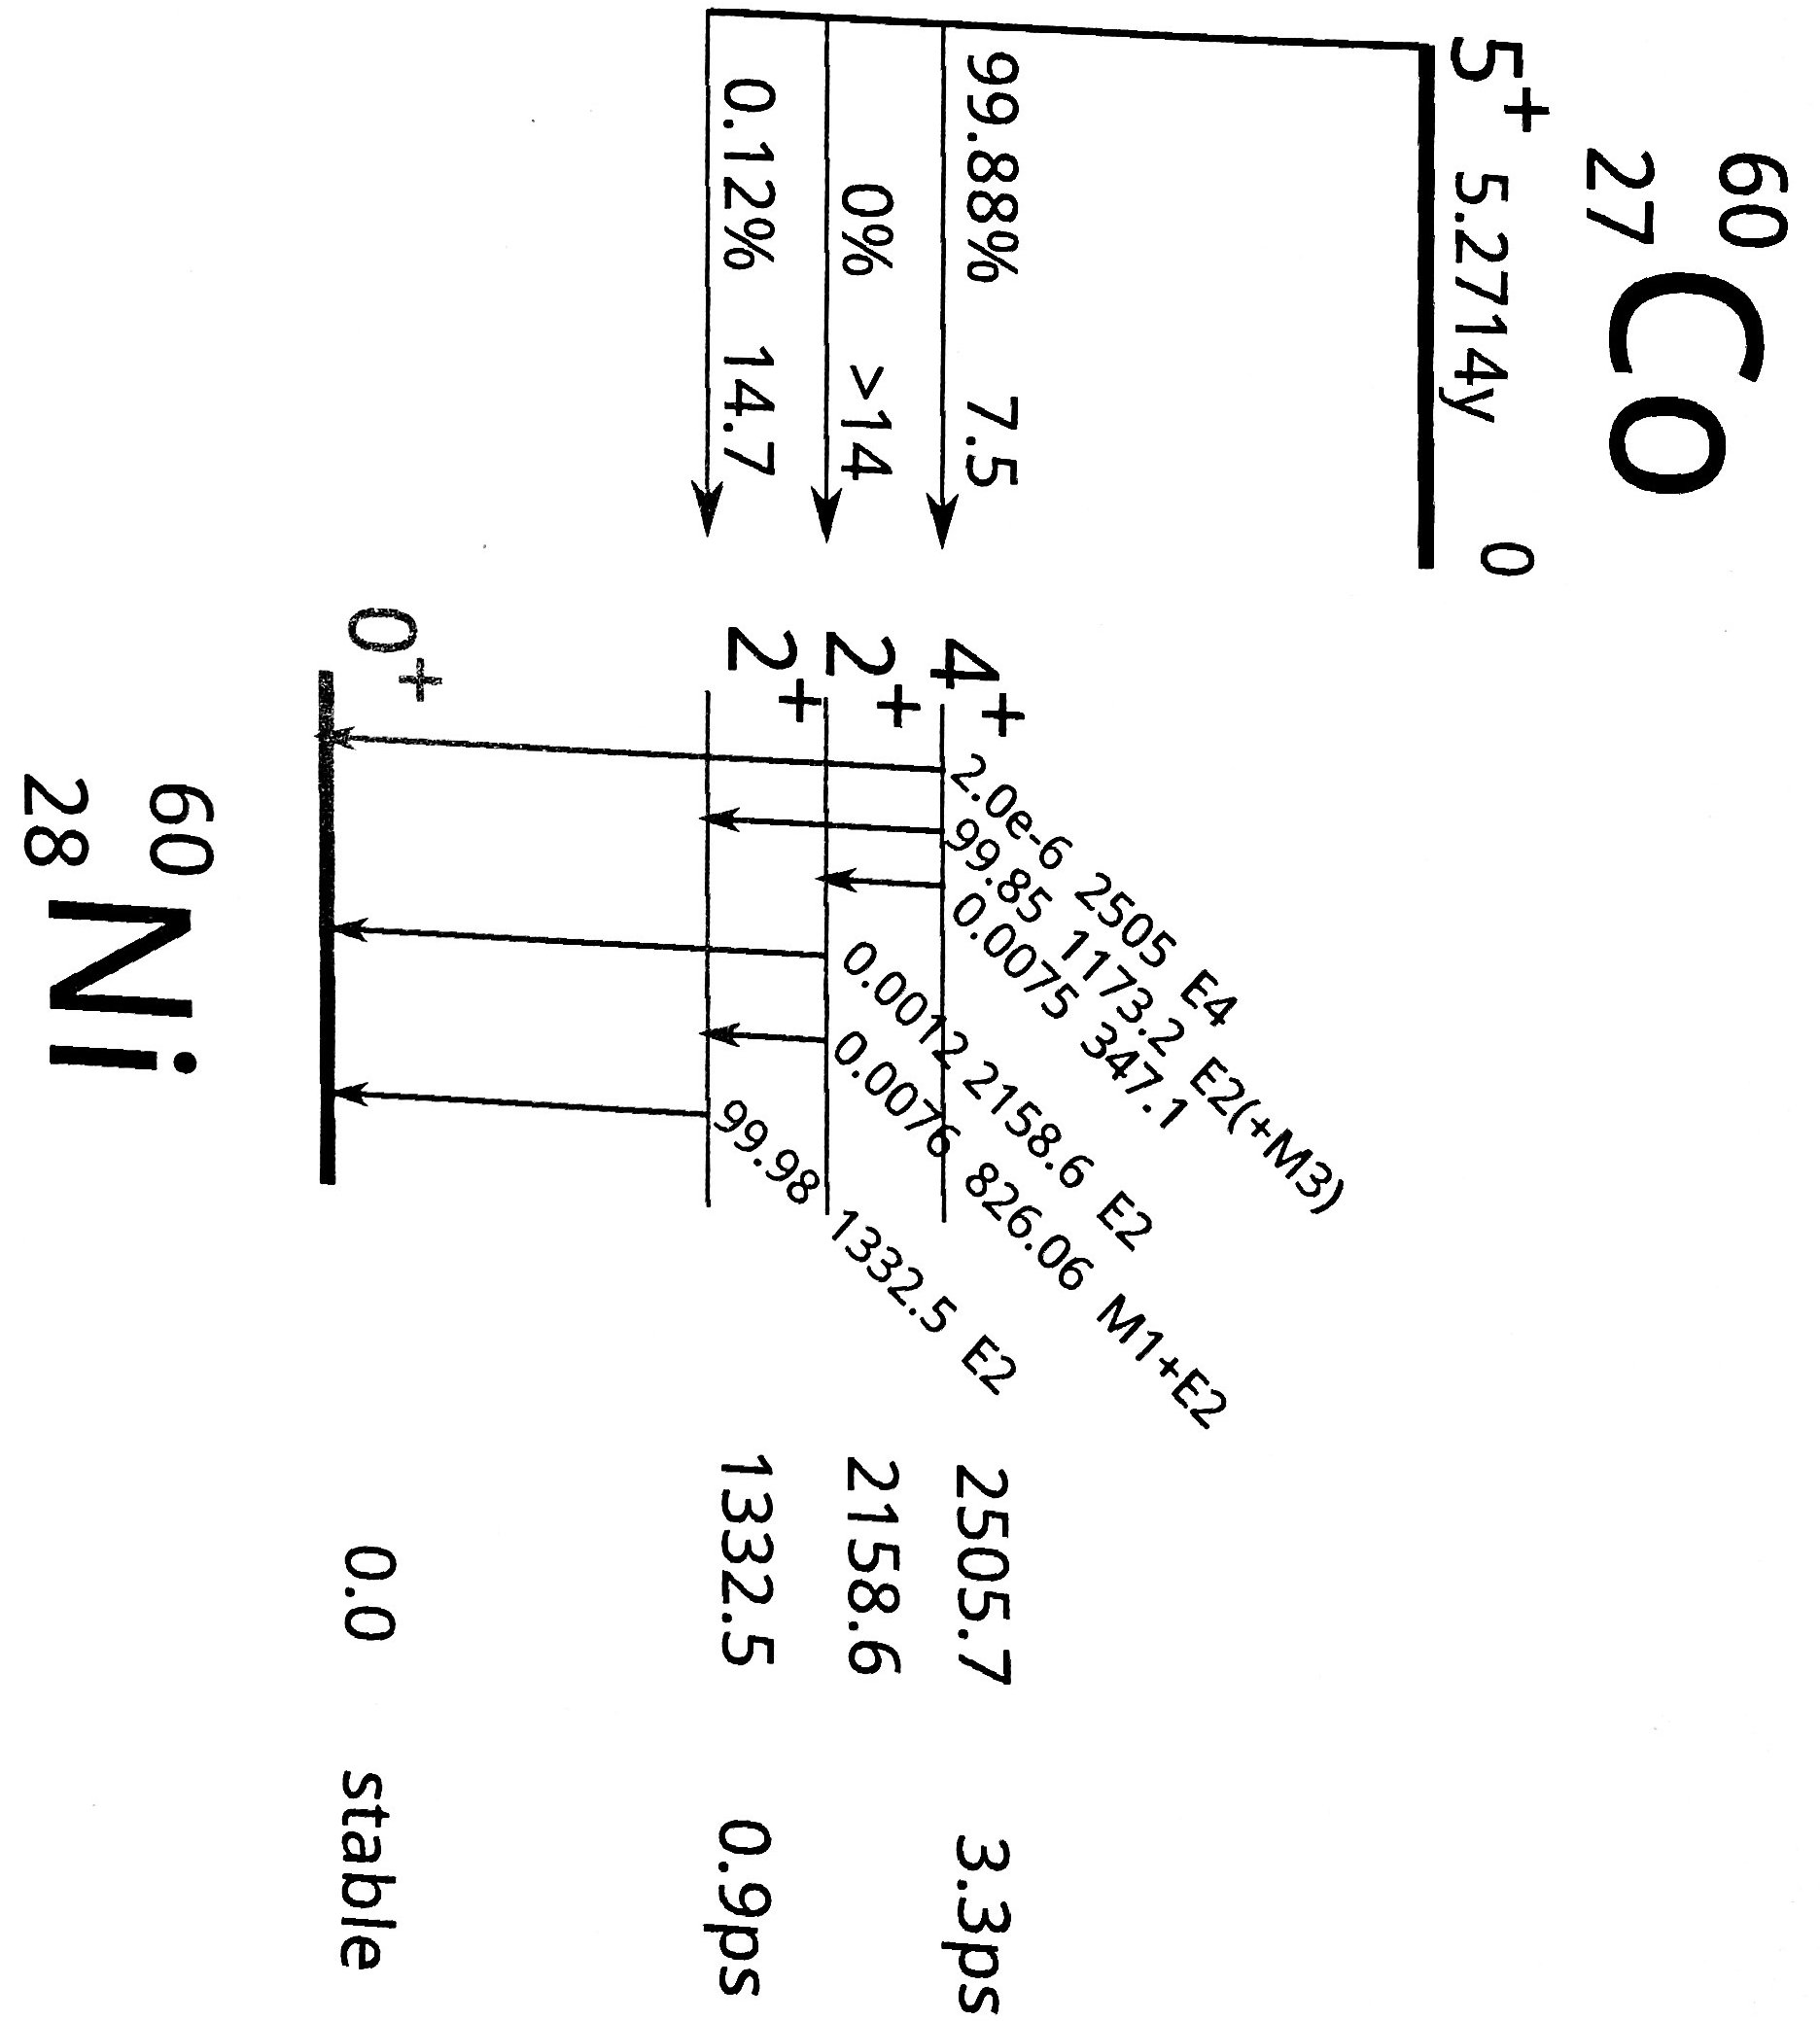
\includegraphics[width=\textwidth, angle=90]{data/co_schema.jpg}
  \end{subfigure}%
  \begin{subfigure}[h]{0.4\textwidth}
    \centering
    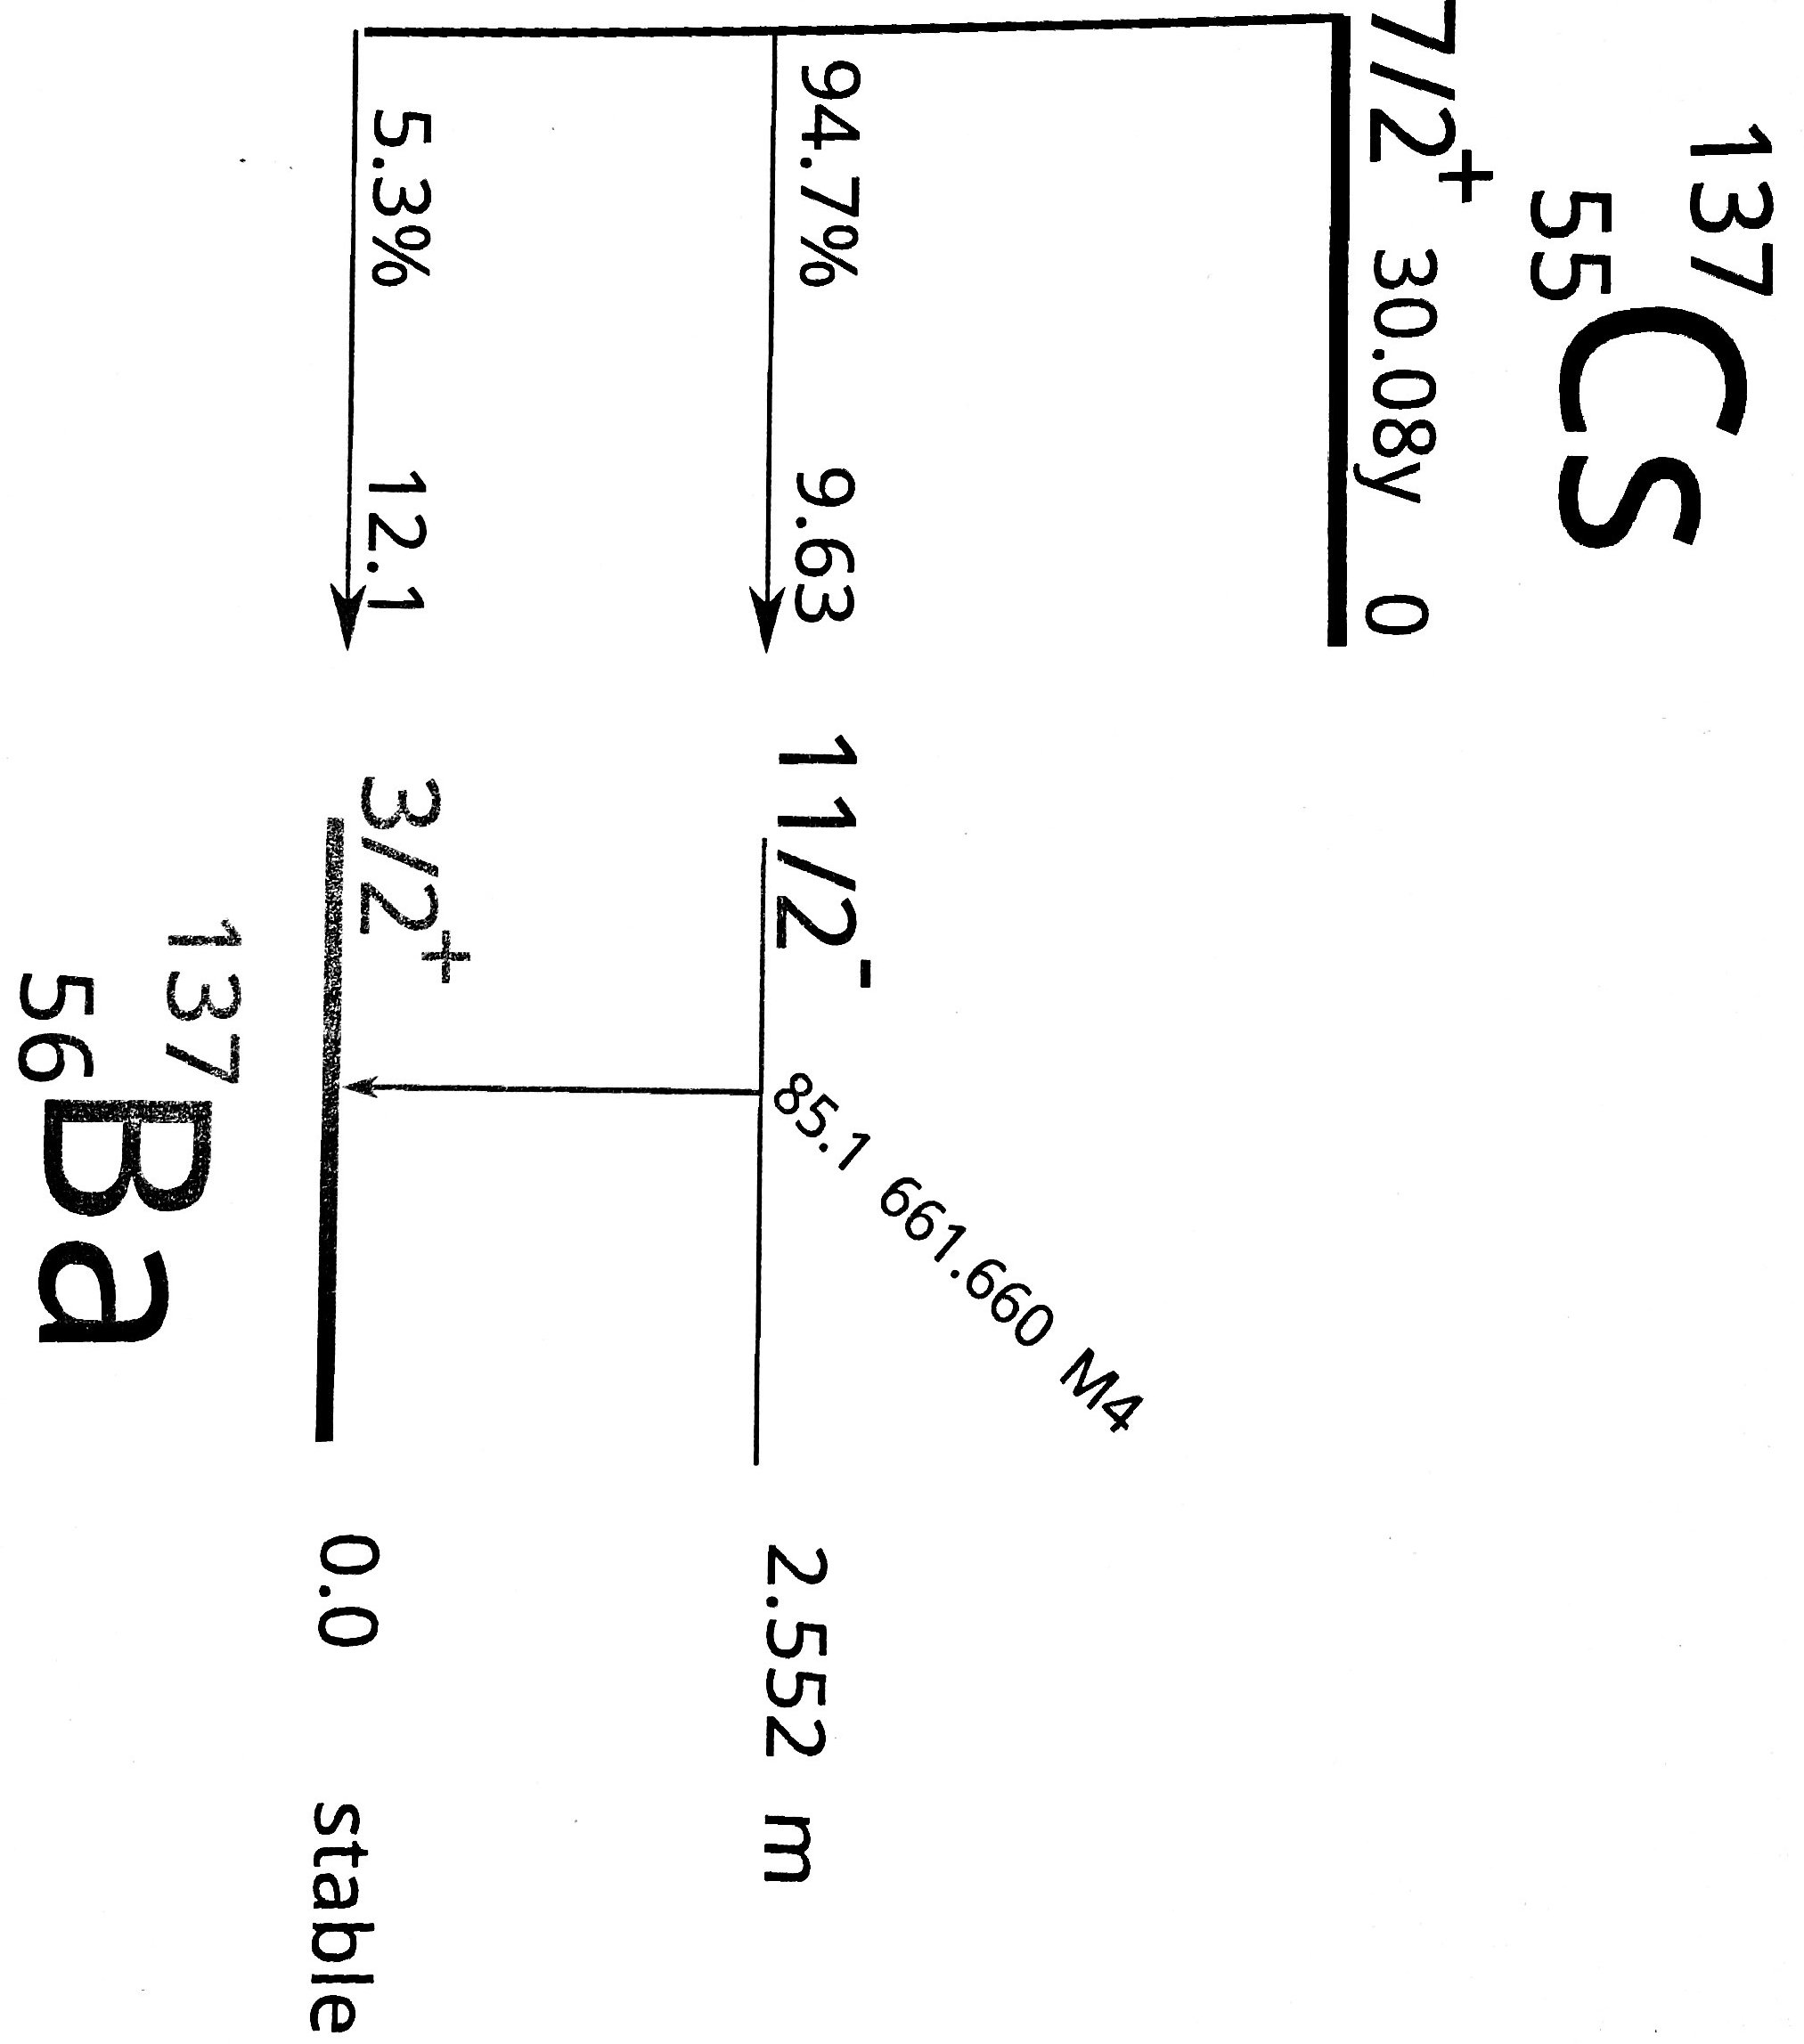
\includegraphics[width=\textwidth,angle=90]{data/cs_schema.jpg}
  \end{subfigure}
  \caption{Zerfallsschemata von Co und Cs aus \cite{praktikumsheft}}
  \label{fig:schema}
\end{figure} 
   
Der Zerfall des Europiums ist komplizierter und deshalb nicht schematisch aufgeführt. Für die Auswertung ist in \cite{praktikumsheft} eine Tabelle mit Gammalinien von Europium aufgeführt.

\subsection{Aktivität der Cs-Probe}
Für die Berechnung der absoluten Peakeffizienz muss die Aktivität der Cs-Probe zum Zeitpunkt des Versuches ermittelt werden. Dafür ist in \cite{praktikumsheft} gegeben, dass im April 1985 die Aktivität bei \SI{9.25e5}{\becquerel} lag. Die Aktivität folgt dem typischen radioaktiven Zerfallsgesetz. Mit der Halbwertszeit von $11018,3 \pm 9,5$ Tagen aus \cite{lebensdauer} folgt somit, dass die Aktivität während des Versuches etwa 
\begin{align*}
  A=\SI{4.3e5}{\becquerel}
\end{align*}
beträgt\footnote{Auf Fehler wird verzichtet, da sie im Vergleich zu den anderen Fehlern bei der Berechnung der absoluten Peakeffizienz vernachlässigbar sind.}.\\

Bei einem Detektor mit runder Stirnfläche mit Durchmesser $d$ im Abstand $R$ zu der Probe folgt Näherungsweise für $R>>d$, dass während einer Zeitdauer $t$
\begin{align}
  N_\mathrm{tot}= \frac{d^2}{16 R^2}At
  \label{eq:ntot}
\end{align}
Gammaquanten auf den Detektor treffen.
